\subsection{Introduction}
The microphone played an important role in this project to detect the 9000 Hz to 10000 Hz sinusoidal sound wave generated by the speaker. Microphone and microphone output types were not steadied before. Background research for microphone was essential to this project. One and half term was spent on researching the project and the microphone to gain good understanding of the project and the hardward. The microphone used in this project was a MEMs microphone. Research of how the MEMs microphones work is explained. Background for digital PDM MEMs microphone (SPH0644LM4H-1) was researched and explained. The conversion of PDM output type to a PCM type was researched and explained. Background for digital I2S MEMs microphone (SPH0644LM4H-B) was researched and explained. The conversion of the I2S output type to PCM was researched and explained. 

The MEMs microphone chosen for this project was not tested before. There was no test to proof of the microphone could work for the distance measurement purpose. Most work of the project has been done on testing the hardware and perform filtering to achieve distance pickup feature of the microphone. A PDM microphone circuit diagram and PCB has been designed while waiting for the breakout board to arrive. A microphone replacement for the I2S breakout board has been performed to swap out the I2S microphone with the PDM microphone. The I2S microphone breakout board was tested. The performance of the I2S microphone was improved with a digital filter and a digital amplifier. The maximum distance measurement was measured. 

In the discussion section below, the difference between the digital PDM MEMs microphone (SPH0644LM4H-1) and the digital I2S MEMs microphone (SPH0644LM4H-B) was discussed. The choice of using the I2S microphone was justified. The choice made for the microcontroller was explained with further improvement. The choise of the filter was justified. The choice of using different gain values for different was justified. The capability of performing distance measurement was discussed.

\subsection{Background research}
\subsubsection{MEMs Microphone}
MEMs \cite{MEMs} stands for microelectro-mechanical systems, a technology that have led to small microphones with high performance. MEMS microphones use acoustic sensors, as shown in Figure \ref{fig:MEMS} below, fabricated on semiconductor production lines using silicon wafers and highly automated processes. Layers of different materials are deposited on top of a silicon wafer. Then the unwanted material is then etched away, creating a moveable membrane and a fixed backplate over a cavity in the base wafer. The sensor backplate is a stiff perforated structure that allows air to move quickly through it. While the membrane is a thin solid structure that flexes in response to the change in air pressure caused by sound waves. Changes in air pressure created by sound waves cause the thin membrane to turn while the thicker backplate remains stationary as the air moves through its perforations. Movements of the membrane create a change between the membrane and the backplate, translated into an electrical signal by the ASIC.

\begin{figure}[H]
	\centering
	\noindent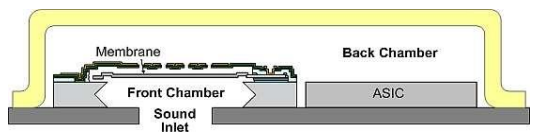
\includegraphics[width=0.8\textwidth]{images/MEMS.png}
	\caption{Cross-section diagram of a typical bottom port MEMS microphone }
	\label{fig:MEMS}
\end{figure}

\subsubsection{Digital PDM output}

Pulse density modulation (PDM) \cite{PDM}, which produces an oversampled single-bit data stream, as shown in Figure \ref{fig:PDM} below. The output of pulse density modulation is proportional to the instantaneous air pressure level. Pulse density modulation is similar to the pulse width modulation (PWM). Pulse density modulation uses a constant pulse width and encodes the signal in the time between pulses. Pulse width modulation uses a constant time between pulses and encodes the signal in the pulse width. 
\begin{figure}[H]
	\centering
	\noindent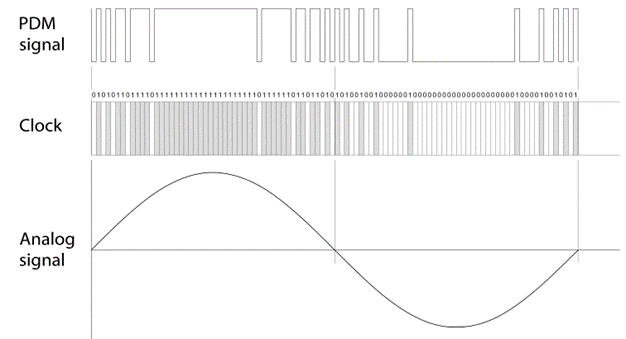
\includegraphics[width=1\textwidth]{images/PDM.png}
	\caption{Sine wave convert to PDM signal with digital output stream}
	\label{fig:PDM}
\end{figure}

\subsubsection{Digital Pulse Density Modulation to Pulse Code Modulation conversion}
To further process the PDM output stream. The best way is to convert the PDM signal into a PCM signal and store in a RAM buffer to be further processed \cite{PDM}. Converting PDM output's 1-bit data stream into PCM samples is accomplished in a digital filtering operation called decimation. The sample rate needs to be reduced by the oversampling factor. It is important that the noise above the audio band in the 1-bit representation is removed. The decimation filters are designed to filter out this noise, leaving only the baseband audio signal. The output of the decimator is a PCM audio stream at the baseband rate. The wordlength increases from 1 bit to around 12 to 16 bits after the filtering.

A decimation filter contains the components as shown in Figure \ref{fig:decimation} below \cite{Decimation}. X(n) represent the microphone's output stream with a frequency of fs. The output of the microphone is feed into an anti-aliasing FIR filter H(z), which is a lowpass filter. To prevent aliasing, the lowpass filter H(z)to suppress contents above fs/2M, which is the Nyquist frequency of the output signal. The filtered signal frequency is then reduced by the oversampling factor M. The decimator pass through every Mth sample and discard the rest of the samples. After the decimator process, the frequency of the filtered signal y(n) is fs/M. 

\begin{figure}[H]
	\centering
	\noindent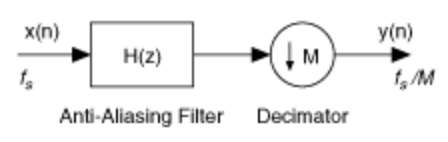
\includegraphics[width=.6\textwidth]{images/decimation.png}
	\caption{Decimation filter components}
	\label{fig:decimation}
\end{figure}

\subsubsection{Digital I2S output}
Inter-IC sound \cite{I2S} is an electrical serial bus interface standard used for connecting audio devices. The output data type is PCM audio data. For I2S protocol, a bit clock line is used for contiunous serial clock, the bit clock for the I2S microphone (SPH0644LM4H-B) was 2.823 MHz, which meant the sampling frequency of the I2S microphone is around 44.1 KHz as shown in Figure \ref{fig:I2Sfreq}; A word select line used for multiple microphone outputs, and considered constant in this project; A data line is used to transfer data in 2's compliment. The the digital I2S protocol, the output raw data of the microphone is already in PCM form and can be analysed straight away.
\begin{figure}[H]
	\centering
	\noindent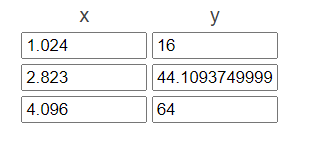
\includegraphics[width=.6\textwidth]{images/I2Sfreq.png}
	\caption{Sampling frequency calculated with interpolation calculator}
	\label{fig:I2Sfreq}
\end{figure}



\subsection{Work Undertaken}
\subsubsection{Design a Microphone breakout}
A microphone breakout board was needed for testing the MEMs PDM microphone. Some breakout board has been ordered, but the shipping time has been extended by the Covid19 situation. With most of the research done, the breakout board was needed as soon as possible for testing. A breakout board was designed as shown in Figure \ref{fig:PDMsche} below. 
\begin{figure}[H]
	\centering
	\noindent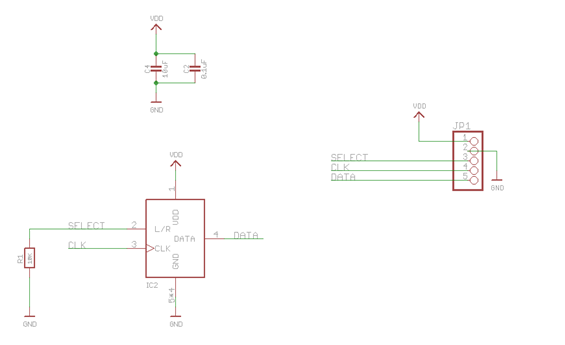
\includegraphics[width=1\textwidth]{images/PDMschematic.png}
	\caption{Schematic of the PDM microphone breakout board}
	\label{fig:PDMsche}
\end{figure}
The PCB of the break has been designed, as Figure \ref{fig:PDMbreakout} shown below, based on the schematic design. The size of the PCB designed was compact to suit the Lab machine at University. The PCB was designed compactly because of the microphone component was not the major function of the prototype, therefore, should not take much space. The through hole of the microphone was limited by the machine, which was bigger then required. the Bigger through hole should not affect the performance of the microphone. 
\begin{figure}[H]
	\centering
	\noindent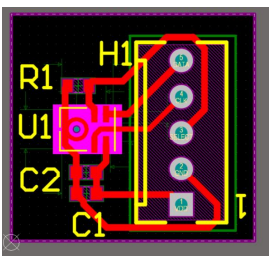
\includegraphics[width=.25\textwidth]{images/PDMbreakout.png}
	\caption{PDM microphone breakout board PCB design}
	\label{fig:PDMbreakout}
\end{figure}

\subsubsection{Modify the I2S breakout board}
A mistake was made when ordered breakout board. The breakout board ordered was the I2S breakout board instead of the PDM microphone breakout board. By comparing the size of the two microphones and the pin layout of the two microphone. It seemed possible to swap out the I2S microphone on the breakout board with the PDM microphone. Figure \ref{fig:modified} below shows the modified breakout board (left) compared to the unmodified breakout board (right). 
\begin{figure}[H]
	\centering
	\noindent\includegraphics[width=1\textwidth]{images/modified.png}
	\caption{PDM microphone breakout board PCB design}
	\label{fig:modified}
\end{figure}
After initialized the modified breakout board correctly, the output of the PDM microphone was 0 constantly. This meant that the microphone was not working. The problem that might have caused this problem was hard to find as the breakout board was modified. The reason could be the microphone was not replaced properly and some connection was not connected properly; The wire was not connected properly; The capacitor was disconnecting properly. The sensitivity of the microphone would decrease after seat in the reflow oven again. There was no point kept trying with the PDM microphone. From comparing the two microphone above, the main difference was the output type and the sensitivity. In both situation, the I2S microphone seemed to be better then the PDM microphone. 

\subsubsection{I2S Microphone Output Testing}
Tests were performed with the I2S microphone breakout board. Hardware testing was implemented first with the output of the microphone connected to a oscilloscope to test the output of the microphone. As shown in Figure \ref{fig:HardwareTest} below, the microphone generated output. The output changed when ambient sound changed (people speaking nearby). 
\begin{figure}[H]
	\centering
	\noindent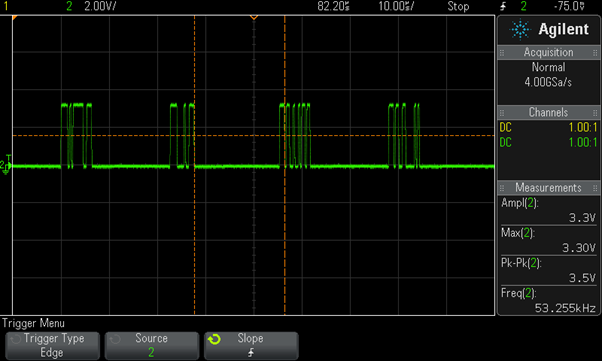
\includegraphics[width=0.7\textwidth]{images/HardwareTest.png}
	\caption{Oscilloscope output of the I2S microphone}
	\label{fig:HardwareTest}
\end{figure}
After the hardware testing proved that the I2S microphone was working. Software testing was performed. RSM function in Teensy audio library was used to analysis the output signal. RSM function scales the raw output of the microphone to between 0 and 1. As shown in Figure \ref{fig:RSM} below, the microphone could detect speaker's 10 kHz tone from 9 cm away in the RMS plot. The plot did not appeared to be sinusoidal. 
\begin{figure}[H]
	\centering
	\noindent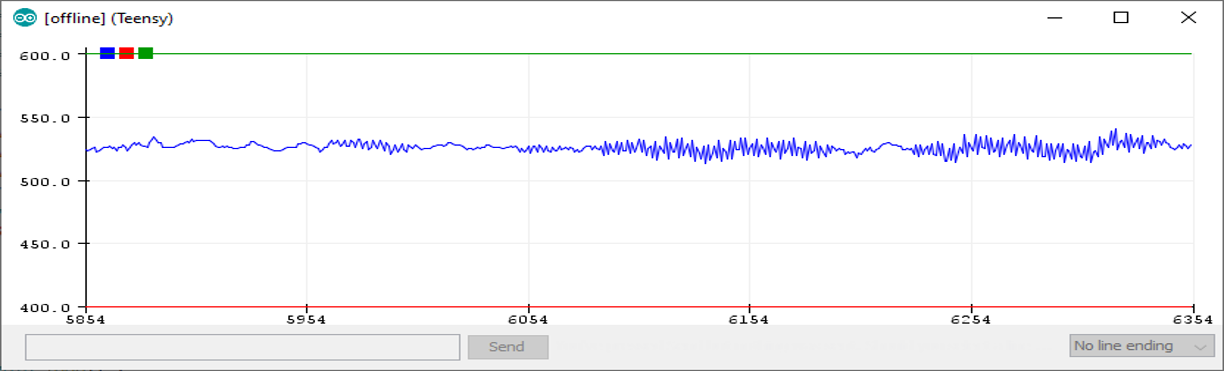
\includegraphics[width=1\textwidth]{images/RSM.png}
	\caption{RMS output of the I2S microphone}
	\label{fig:RSM}
\end{figure}
A Fast Fourier Transform function was then used to analysis the different frequency component in the microphone's output signal. From the FFT analysis, a low frequency component was noticed in the system. A high pass filter was then used to filter out the frequency component less then 100 Hz. A high pass filter was used to filter the output signal. The filter was a second order biquad IIR filter. After the filter was implemented, the frequency component was filtered out. As Figure \ref{fig:FFT} shown below, the left picture was the unfiltered signal FFT with each column represent 47 Hz range. The right picture shown the filtered signal FFT with no value on the left two columns. 

\begin{figure}[H]
	\centering
	\noindent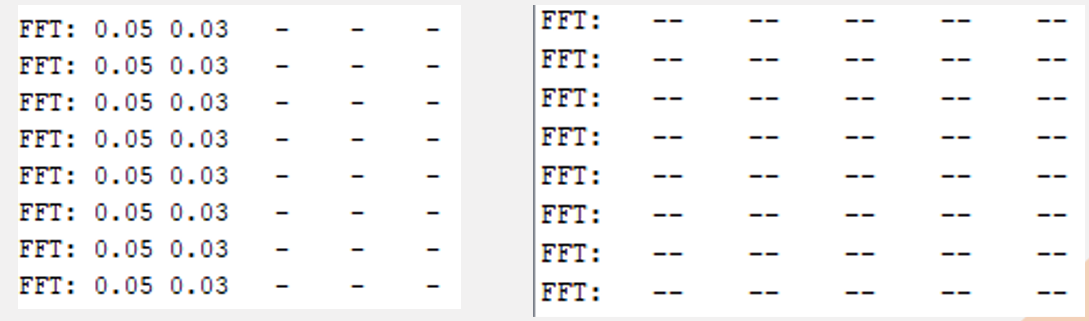
\includegraphics[width=1\textwidth]{images/FFT.png}
	\caption{FFT of the microphone output without/with filter}
	\label{fig:FFT}
\end{figure}
A digital amplifier was used to amplify the filtered output signal to increase the frequency. Amp function was used with a gain set up. The gain value of the amplifier affected the sensitivity of the microphone. In the FFT function, each column of the serial output represented a frequency range of 47 Hz with the number represented the magnitude of the output. Figure \ref{fig:gain} below showed that filter gain value affect the magnitude of the output signal. The microphone and the speaker were placed 30 cm apart in a quite environment (late night). FFT function was used to generate the output magnitude for 10 KHz sound. 
\begin{figure}[H]
	\centering
	\noindent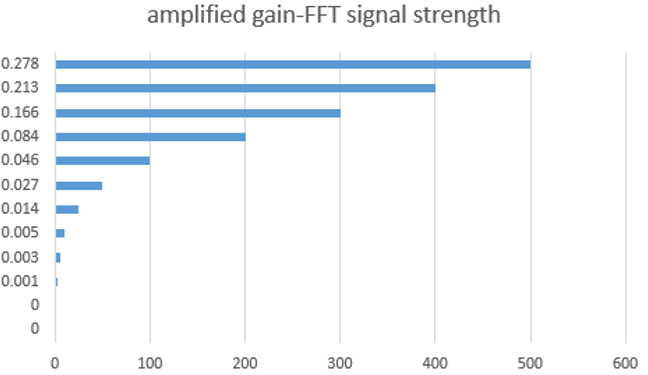
\includegraphics[width=1\textwidth]{images/Gain.png}
	\caption{FFT output 10KHz signal strength affected by amplifier gain }
	\label{fig:gain}
\end{figure}
With amplifier gain of 10, the FFT could detect the speaker's 10KHz sound from 25 meters away in a quiet but echoed environment. The ambient noise component contain air conditioning, computers. With a gain of 5, the FFT function could detect the speaker's 10KHz sound from 10 meters away in a noisy lab environment (Day time university lab). The ambient noise contained people talking, computer, air conditioning, keyboard typing and mouse clicking. The main code mentioned in this section can be found in Microphone Code Appendix.  




\subsection{Discussion}
\subsubsection{Why I2S microphone is better then the PDM microphone for the project}
This microphone was good for this project because of its small dimension of 3.5mm x 2.65mm x 0.98mm (L x W x H) and the breakout board's dimension is 16.7mm x 12.7mm x 1.8mm. Both I2S microphone and the PDM microphone was the same size. As shown in Figure \ref{fig:I2S} below, the breakout board of the I2S microphone with the center component being the MEMs I2S microphone. Small size microphone benefit the prototype by minimizing the size, which reduce the manufacture cost of the prototype and reduce further packaging cost of the prototype. 
\begin{figure}[H]
	\centering
	\noindent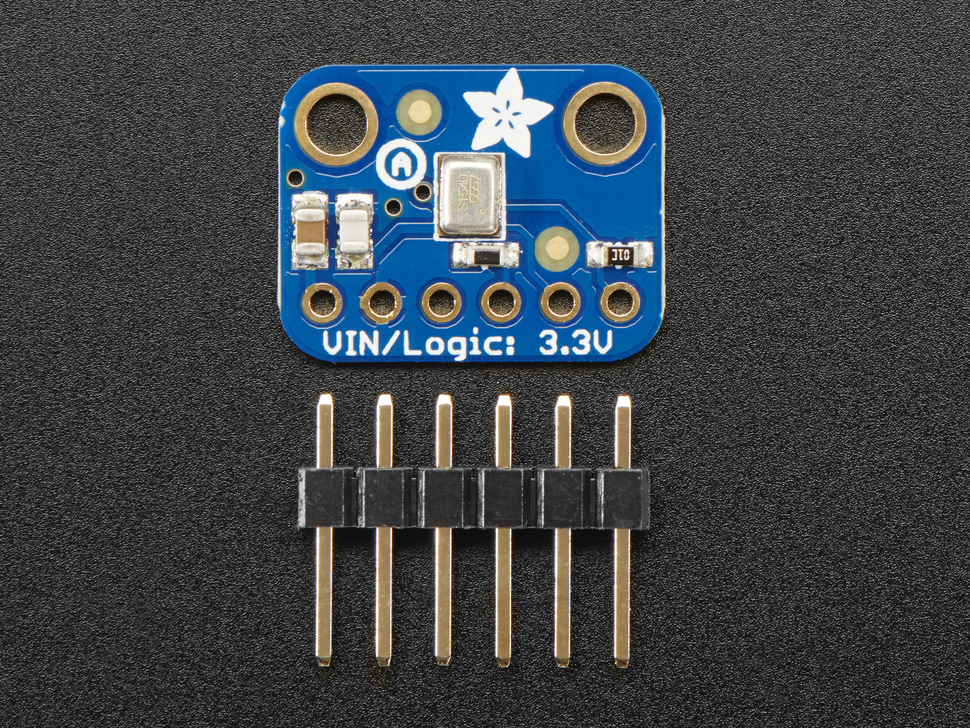
\includegraphics[width=0.5\textwidth]{images/I2S.jpg}
	\caption{Digital I2S MEMs Microphone Breakout Board }
	\label{fig:I2S}
\end{figure}
Both I2S microphone and the PDM microphone were omnidirectional. Omnidirectional microphone receives sound from all surrounding environment. The I2S microphone has the sensitivity of -26 dBFS which is a distance pick microphone. The PDM microphone has the sensitivity of -37 dBFS which is also a distance pick up microphone. The I2S microphone has the better sensitivity to detect the speaker from further away.

\subsubsection{Microcontroller used to test the microphone}
The microcontroller used in this project to test the microphone was a teensy 4.0. High clock frequency was the reason teensy 4.0 was chosen. 600MHz clock frequency was much faster compared to the 32-bit ARM CortexTM M4F CPU used in the actual prototype (nRF52840) which has the clock frequency of 80MHz. The clock frequency of the teensy can be slow down to match the CortexTM M4F CPU to test its maximum performance. 
\subsubsection{Microcontroller Improvments}
The problem with using teensy 4.0 was that it was not built mainly for audio devices. An audio shield would make testing the microphone easier. Due to the lockdown, an audio shield was not ordered. With an audio shield, the output of the microphone can be saved in a SD card and the data can be played back and analysed. The audio library of teensy was difficult to understand and to use. Some function was half built or not working properly. Arduino Zero is made for audio devices. It has fully built audio library. But the clock frequency of the Arduino Zero is 48 MHz.

\subsubsection{RMS function}
The RMS function was only detecting the 10KHz tone 9cm away. The problem was that the microphone's output frequency was 44.1KHz, but the RMS function plot was only generating 100 samples per second, which was not close to Nequist frequency for detecting the 10KHz sound. With method mentioned in Aryan's section with plotting the raw output data, the signal showed sine wave when the speaker was playing near it, the code is listed in Test Code Appendix. Which proves that the microphone was working, but the RMS function was not suitable for analyzing the microphone's output.  

\subsubsection{Highpass filter}
From the RMS function plot, where the graph was not centered at 500, but at 540. The FFT function plot where the 0Hz to 94Hz component was always detected something. This proves that there was a DC component in the microphone's output. Therefore, a highpass filter was used to filter out the low frequency component (less then 30Hz). This filter cleared the 0 to 94 Hz component in the FFT plot.

\subsubsection{Digital amplifier gain}
The gain of the amplifier could increase the range that microphone picks up the speaker significantly, from 9 cm to 25 meters. The use of the gain values depended on the level of ambient noise level. In a quiet environment with little amount of ambient noise, the gain can be set to 500 and with no interference by the noise. In a noisy environment with high level of ambient noise, the gain of 10 would cause noise to be amplified high enough to affect the 10KHz FFT output. The maximum distance the microphone could successfully detect in a quiet environment (late night) with a gain of 10 was 25 meters. This distance could be beaten with a gain of 500 in a quieter space, but not practical in an office environment. This measurement provided the maximum distance of 25 meters that distance measurement can be performed in an office like environment. This satisfied the requirement of this project for maximum distance measurement.


\subsubsection{Perform distance measurement with FFT function}
One of the simplest way to perform distance measurement for initial testing was connected two teensy with a wire to synchronize the time. When the speaker started display sound, it also pulls the wire high. The time difference between the wire pulled high and the FFT function detected the signal would be the time sound wave has traveled. The difficult in this case was the FFT function not sampled fast enough. The time between two FFT samples was 0.011 second. This sampling frequency caused the distance measurement contain an uncertainty of 3.773 meters. 





